\documentclass[../main]{subfiles}

\begin{document}

\clearpage

\setcounter{eqnarray}{0}
\setcounter{equation}{0}
\setcounter{figure}{0}

\part*{第8回}

\subsection{Biot-Savartの法則}
\begin{itembox}[c]{ベクトル積(外積)}
\begin{equation*}
{\bf a}= \left(
\begin{array}{l}
a_x \\
a_y \\
a_z
\end{array}
\right)
,
{\bf b}= \left(
\begin{array}{l}
b_x \\
b_y \\
b_z
\end{array}
\right)
\quad
{\bf a} \times {\bf b} =\left(
\begin{array}{l}
a_yb_z-a_zb_y \\
a_zb_x-a_xb_z \\
a_xb_y-a_yb_x
\end{array}
\right)
\end{equation*}
\end{itembox}

\begin{equation*}
\nabla =\left(
\begin{array}{l}
\frac{\partial}{\partial x} \\
\frac{\partial}{\partial y} \\
\frac{\partial}{\partial z}
\end{array}
\right)
\mbox{とすると}
{\rm rot}\,{\bf A}= \nabla \times {\bf A}
\end{equation*}
性質1 \\
\begin{equation*}
{\bf a} \times {\bf b} = -{\bf b} \times {\bf a}
\end{equation*}
とくに,${\bf b} = k{\bf a}$ならば,
\begin{equation*}
{\bf a} \times {\bf b} = k({\bf a} \times {\bf a}) = -k({\bf a} \times {\bf a}) ={\bf 0}
\end{equation*}
性質2 \\
\begin{eqnarray*}
{\bf a} \cdot ( {\bf a} \times {\bf b} ) &=& a_x(a_yb_z-a_zb_y) \\
&+&a_y(a_zb_x-a_xb_z) \\
&+&a_z(a_xb_y-a_yb_x) = {\bf 0}
\end{eqnarray*}
同様に${\bf b} \cdot ( {\bf a} \times {\bf b} )=0$となり,${\bf a} \times {\bf b}$は${\bf a}$とも${\bf b}$とも直交することがわかる.\\
性質3 \\
${\bf a}$と${\bf b}$のなす角を$\theta$とすると,
\begin{eqnarray*}
|{\bf a} \times {\bf b}|=|{\bf a}||{\bf b}|\sin\theta \quad (0 \leq \theta \leq \pi) \\
|{\bf a} \times {\bf b}|^2 + |{\bf a} \cdot {\bf b}|^2 = |{\bf a}|^2|{\bf b}|^2(\sin^2\theta + \cos^2\theta)=|{\bf a}|^2|{\bf b}|^2
\end{eqnarray*}
$|{\bf a} \times {\bf b}|$は${\bf a}$と${\bf b}$のなす平行四辺形の面積となっている.
\\
\newpage
さて,定常電流があると静磁場が生じるが,それを定式化したい.以下,簡単のため定常電流を線電流として議論をする. \\
微小区間の線電流が離れた微小な場所に生じさせる磁場について考える. \\
${\bf dl}$は微小であるから,位置${\bf r}$と${\bf dl}$の距離は一定であるとみなしてよい. \\
\begin{figure}[h]
 \begin{center}
  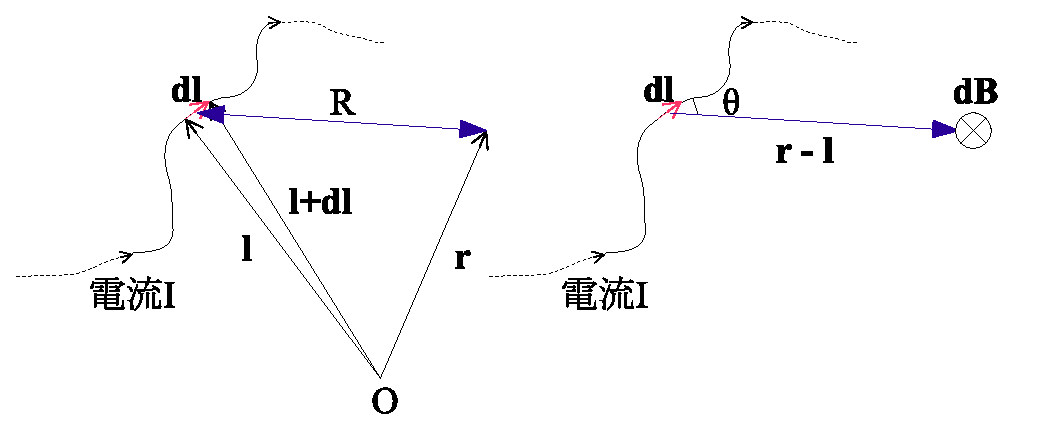
\includegraphics[width=150mm]{8.1.eps}
 \end{center}
 \caption{}
 \label{fig:one}
\end{figure}
大きさ
\begin{eqnarray*}
|{\bf dB}|=\frac{\mu_0 {\rm I}}{4 \pi}\frac{|{\bf dl}\sin\theta|}{R^2}=\left| \frac{\mu_0 {\rm I}}{4 \pi}\frac{{\bf dl} \times ({\bf r}-{\bf l})}{|{\bf r}-{\bf l}|^3} \right|
\end{eqnarray*}
向き \\
\begin{center}
$\bigotimes$
\end{center}
大きさと向きの両方を含む式は,
\begin{eqnarray*}
{\bf dB}=\frac{\mu_0 {\rm I}}{4 \pi}\frac{{\bf dl} \times ({\bf r}-{\bf l})}{|{\bf r}-{\bf l}|^3}
\end{eqnarray*}
これを線電流にそって線積分したものが,位置${\bf r}$における線電流によって生じる磁場である.
\begin{itembox}[c]{Biot-Savartの法則}
\begin{eqnarray}
{\bf B}({\bf r})=\frac{\mu_0 {\rm I}}{4 \pi} \int_{C}^{}\frac{{\bf dl} \times ({\bf r}-{\bf l})}{|{\bf r}-{\bf l}|^3}
\end{eqnarray}
$\frac{\mu_0}{4 \pi} = 10^{-7} {\rm [NA^{-2}]}$:真空の透磁率 \\
${\bf B} \mbox{磁束密度} {\rm [T]=[NA^{-1}m^{-1}]=[Wbm^{-2}]=[JA^{-1}m^{-2}]=[10^4gauss]} $
\end{itembox}
\newpage
{\bf 例1:直線電流} \\
\begin{figure}[htbp]
 \begin{center}
  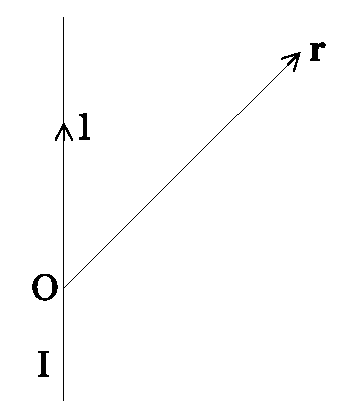
\includegraphics[width=30mm]{8.2.eps}
 \end{center}
 \caption{}
 \label{fig:two}
\end{figure}
\begin{eqnarray*}
{\bf dl}=(0,0,dl) \\
{\bf r}-{\bf l}=(x,y,z-l)
\end{eqnarray*}
\begin{eqnarray*}
{\bf dl} \times ({\bf r}-{\bf l}) =\left(
\begin{array}{l}
0 \\
0 \\
dl
\end{array}
\right)
\times
\left(
\begin{array}{l}
x \\
y \\
z-l
\end{array}
\right)
=
\left(
\begin{array}{l}
-ydl \\
xdl \\
0
\end{array}
\right)
\end{eqnarray*}
\begin{eqnarray*}
{\bf B}({\bf r})&=&\frac{\mu_0 {\rm I}}{4 \pi} \int_{- \infty}^{\infty}\frac{{\bf dl} \times ({\bf r}-{\bf l})}{|{\bf r}-{\bf l}|^3} \\
&=& \frac{\mu_0 {\rm I}}{4 \pi} \int_{- \infty}^{\infty}\frac{1}{\left( x^2+y^2+(z-l)^2 \right)^{\frac{3}{2}}}
\left(
\begin{array}{l}
-ydl \\
xdl \\
0
\end{array}
\right)
\end{eqnarray*}
ここで $l=z+(x^2+y^2)^{\frac{1}{2}}\tan\theta$とおくと
\begin{eqnarray*}
\int_{- \infty}^{\infty}\frac{dl}{\left( x^2+y^2+(z-l)^2 \right)^{\frac{3}{2}}} = \frac{1}{x^2+y^2} \int_{- \frac{\pi}{2}}^{\frac{\pi}{2}} \cos\theta d\theta = \frac{2}{x^2+y^2}
\end{eqnarray*}
となるから,
\begin{eqnarray*}
{\bf B}({\bf r})&=&\frac{\mu_0 {\rm I}}{2 \pi}
\left(
\begin{array}{l}
\frac{-y}{x^2+y^2} \\
\\
\frac{x}{x^2+y^2} \\
\\
0
\end{array}
\right)
\end{eqnarray*}
\begin{figure}[h]
 \begin{center}
  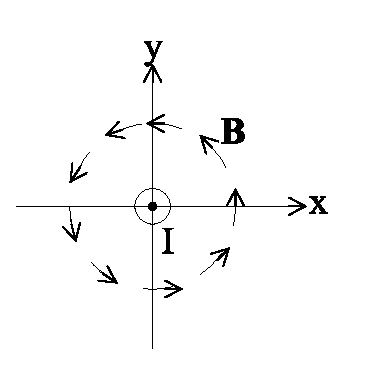
\includegraphics[width=30mm]{8.3.eps}
 \end{center}
 \caption{}
 \label{fig:three}
\end{figure}
\newpage
{\bf 例2:円電流} \\
\begin{figure}[htbp]
 \begin{center}
  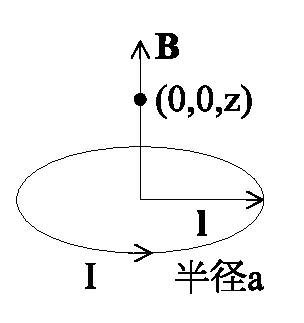
\includegraphics[width=50mm]{8.4.eps}
 \end{center}
 \caption{}
 \label{fig:four}
\end{figure}
中心軸上の位置${\bf r} = (0,0,z)$ での${\bf B}$を求める.
\begin{eqnarray*}
{\bf l} = (a \cos\theta,a\sin\theta,0) \\
{\bf dl} = (-a \sin \theta d\theta,a \cos \theta d\theta,0) \\
{\bf r}-{\bf l}=(-a \cos\theta,-a\sin\theta,z) \\
\end{eqnarray*}
\begin{eqnarray*}
{\bf dl} \times ({\bf r}-{\bf l}) = \left(
\begin{array}{l}
-a \sin \theta d\theta \\
\\
a \cos \theta d\theta \\
\\
0
\end{array}
\right)
\times
\left(
\begin{array}{l}
-a \cos\theta \\
\\
-a\sin\theta \\
\\
z
\end{array}
\right)
=
\left(
\begin{array}{l}
za \cos\theta d\theta \\
\\
za \sin\theta d\theta \\
\\
a^2 d\theta
\end{array}
\right)
\end{eqnarray*}
\begin{eqnarray*}
{\bf B}({\bf r})=\frac{\mu_0 {\rm I}}{4 \pi} \int_{0}^{2 \pi} \frac{1}{(a^2+z^2)^{\frac{3}{2}}}
\left(
\begin{array}{l}
za \cos\theta d\theta \\
\\
za \sin\theta d\theta \\
\\
a^2 d\theta
\end{array}
\right)
=
\frac{\mu_0 {\rm I}}{4 \pi}
\left(
\begin{array}{l}
0 \\
\\
0 \\
\\
2 \pi a^2
\end{array}
\right)
=
\left(
\begin{array}{l}
0 \\
\\
0 \\
\\
\frac{\mu_0 {\rm I}a^2}{2 (a^2+z^2)^{\frac{3}{2}} }
\end{array}
\right)
\end{eqnarray*}
\newpage
{\bf 例3:ソレノイド} \\
\begin{figure}[htbp]
 \begin{center}
  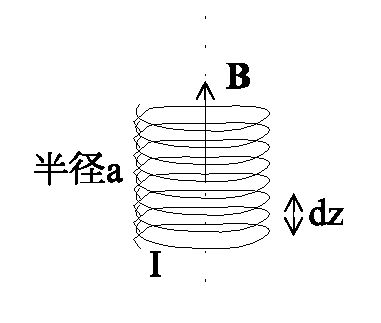
\includegraphics[width=50mm]{8.5.eps}
 \end{center}
 \caption{}
 \label{fig:five}
\end{figure}
半径a,単位長さあたりの巻き数nのソレノイドについて,中心軸上の磁束密度の大きさ$B$を求める.
すると例2の結果のz成分について,${\rm I}$を${\rm I}ndz$に置き換えて$-\infty$から$\infty$まで積分すればよいので,
\begin{eqnarray*}
B=\int_{-\infty}^{\infty} \frac{\mu_0 a^2  {\rm I}ndz  }{2 (a^2+z^2)^{\frac{3}{2}} }
\end{eqnarray*}
$z=a\tan\theta$とおくと,
\begin{eqnarray*}
B= \frac{\mu_0 {\rm I}n}{2} \int_{-\frac{\pi}{2}}^{\frac{\pi}{2}} \cos \theta d\theta = \mu_0 {\rm I}n
\end{eqnarray*}
\\
さて,2.1節で定義した電流密度を用いて,Biot-Savartの法則を書き換える.
電流密度${\bf i}={\bf i}({\bf r})$が与えられているとき,
位置${\bf r'}$まわりについて,電流と電流密度の関係は微小体積$d{\bf r'}$\footnote{記号として紛らわしいが,これはスカラー量なので注意されたい.}
を用いて以下のように書き直せる.
\begin{eqnarray*}
{\rm I}{\bf dl} = {\bf i}({\bf r'})d{\bf r'}
\end{eqnarray*}
すると式(1)の電流密度を用いた表記が得られる.
\begin{itembox}[c]{Biot-Savartの法則}
\begin{eqnarray}
{\bf B}({\bf r})=\frac{\mu_0}{4 \pi} \int_{V}^{}\frac{{\bf i}({\bf r'}) \times ({\bf r}-{\bf r'})}{|{\bf r}-{\bf r'}|^3} d{\bf r'}
\end{eqnarray}
\end{itembox}
\end{document}

